\section{Pauvreté monétaire et pauvreté multidimensionnelle : analyse croisée}
\label{ann:D}

La pauvreté monétaire (seuil ANSD~: 757\,FCFA/jour, EHCVM 2018-2019
\parencite{ansd2022}) et la pauvreté N-MODA mesurent des réalités partiellement
non superposables, ce qui justifie leur usage complémentaire.

Le croisement des deux mesures, sur les enfants de 0 à 17 ans de l'EHCVM I,
distingue quatre profils~: non pauvres selon les deux approches (31,7\,\%),
doublement pauvres (28,2\,\%), pauvres monétaires non multidimensionnels
(4,7\,\%, accès possible à des biens hors marché), et pauvres
multidimensionnels non monétaires (35,5\,\%, souvent ruraux, invisibles à la
mesure monétaire seule).

Cette proportion de 35,5\,\% d'enfants « invisibles » à la mesure monétaire
justifie l'intégration des indicateurs N-MODA dans les outils de ciblage des
programmes sociaux sénégalais.

\begin{figure}[H]
  \centering
  \caption{Diagramme de Venn : pauvreté monétaire et N-MODA (EHCVM I, 2018-2019)}
  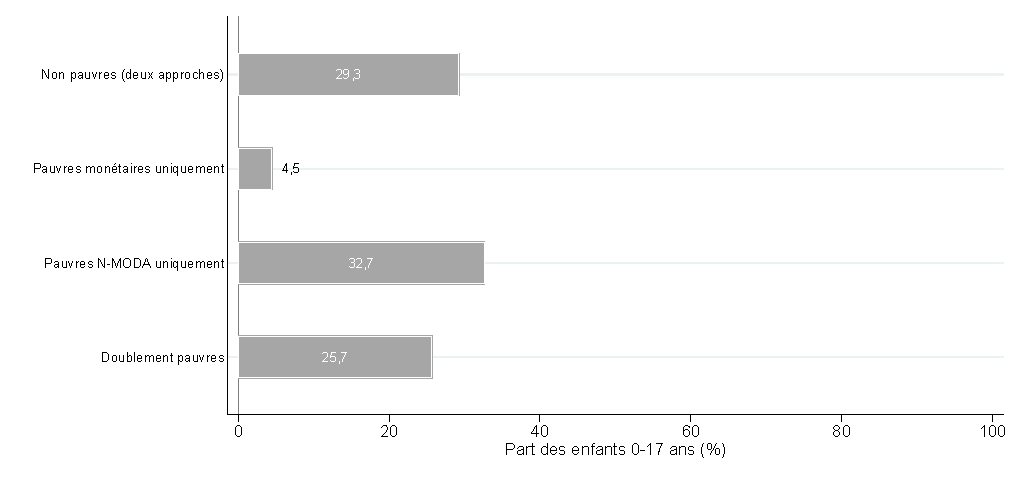
\includegraphics[width=0.75\linewidth]{figures/fig_croisement_pauvrete.pdf}
  \label{fig:venn_pauvrete}
\end{figure}
